\chapter{Croissance et environnement}
\section{La croissance et l'environnement}
\subsection{Les 3 piliers dde la croissance}
\begin{itemize}
    \item \textbf{L'innovation} \footnote{Progrès technique}
    \item \textbf{L'éducation} \footnote{Capital humain}
    \item \textbf{Les ressources naturelles} \footnote{Empilement des ressources primaires  et croissancde de la consommation d'énergie}
\end{itemize}
\subsection{Les conséquences de la croissance}
\begin{itemize}
    \item La soutenabilité de la dette
    \item L'emploi
    \item La pauvreté
    \item La qualité de l'environnement 
\end{itemize}
\newpage
\subsubsection{Constat}
Les biens environnementaux sont des biens rivaux et non-exclusifs alors que le climat est un bien non-rival et non-exclusif. \newline
$\implies$ le marché est défaillant à travers les externalités négatives : les ressources naturelles sont limités et posent des problèmes de \textbf{régénération}
\subsubsection{Conséquences}
On s'attend à avoir une baisse de la croissance, une diminution de la qualité de vie environnementale et de la perte de bien-être
\section{Faits stylisés}
\begin{itemize}
    \item 1,1 milliard d’être humains vivent avec moins d’1 dollar par jour
    \item Près de 3 milliards d’êtres humains vivent avec moins de 2  dollars par jour
    \item Le PIB \footnote{Mesure de la qualité de l'économie d'un pays, d'une entreprise ou d'un particulier} entre chaque pays varie énormément et n'est pas constant dans le temps  
    \item Les revenus par tête pour la plupart des pays ont augmentés mais des disparités s'amplifient
\end{itemize}
\newpage
\section{Les nouvelles théories de la croissance}
\subsection{La nouvelle économie \& Paul Romer}
Apparue dans les années 90s avec les NTIC \footnote{Nouvelles technologies de l(information et de la Communication)}, cette "nouvelle économie" marque une reprise de croissance énorme grâce aux nouvelles technologies comme par exemple : USA \newline
Romer explique que le taux de croissance peut être endogène \footnote{provoque des problèmes en interne} et qu'il faut privilégier la croissance grâce à la R\&D et à l'éducation
\subsection{Objectifs Européens de Lisbonne (mars 2000)}
Faire de l'économie de l'UE une économie de connaissance dynamique compétitive
\subsection{Objectifs Européens de Barcelone (mars 2002)}
Renforcer la R\&D
\section{Education et innovation}
\subsection{Education et croissance}
Les moyens d'acquisition des connaissances sont :
\begin{itemize}
    \item l'\textbf{imitation} : permet d’atteindre la frontière de la période précédente \footnote{On parle ici de frontières technologiques}
    \item l'\textbf{innovation} : c’est améliorer la technologie : c’est donc faire bouger cette frontière
\end{itemize}
\newpage
\begin{figure}[hbt!]
    \centering
    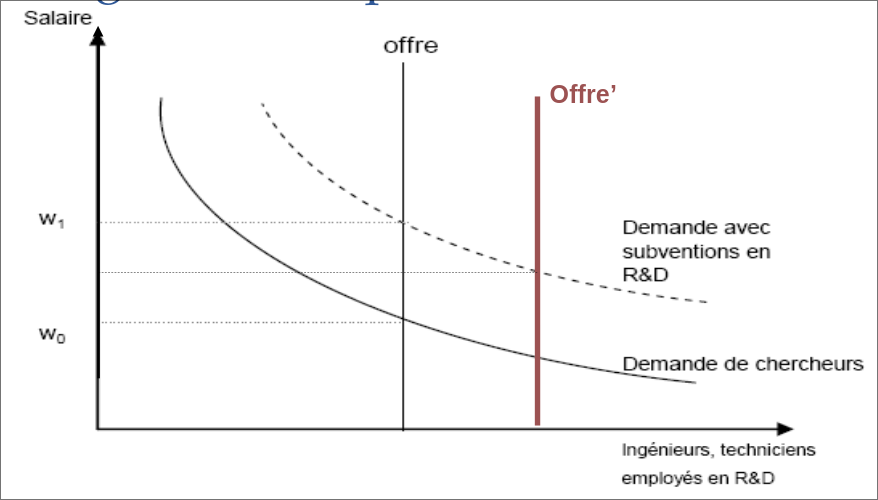
\includegraphics[scale=0.3]{Pics/innovation_enseingment_sup.png}
\end{figure}
\section{Économie de l’environnement et des ressources naturelles}
\subsection{La courbe environnementale de Kuznets}
\begin{figure}[hbt!]
    \centering
    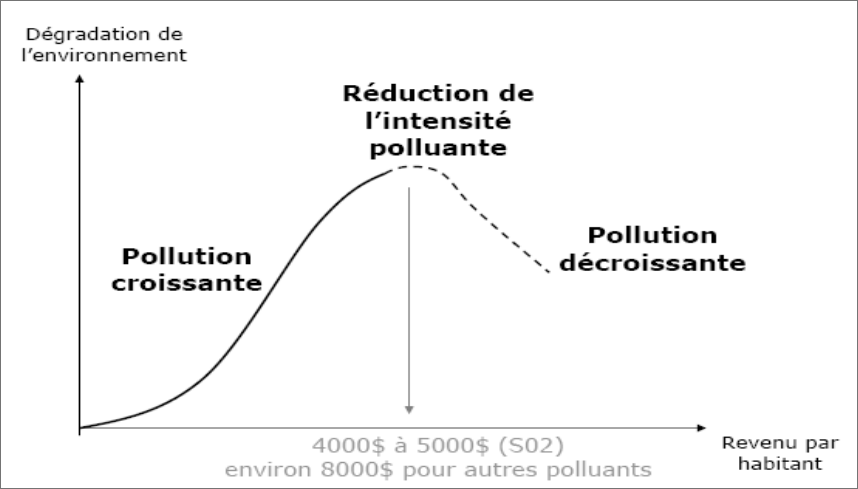
\includegraphics[scale=0.3]{Pics/courbe_environnementale_de_Kuznets.png}
    \caption{Courbe environnementale de Kuznets : dès un seuil de revenus dépassé, il y aurait un découplage pollution/richesse}
\end{figure}